
\section{App architecture}
\label{sec:app-architecture}

Sweetie could be a long terms project with new extensions in the future so we concentrate a lot of effort to take and maintain a certain architecture in order to keep maintainability and extendability of the app.

Today in the Android community Model View Presenter architecture pattern is the major suggest architecture pattern although the MVP is not a complete architecture pattern as Uncle Bob said in numerous of his talks [].  By the way we would like to clarify that the official Android designer Dianne Hackborn \cite{Dianne_Hackborn_android_arch} doesn't give a precise architecture, Android components by design could be use in very different architecture styles.

In fact the MVP in Android is an element of the Clean Architecture explained very well by his inventor Uncle Bob []. You could see this from the many examples grouped by android community in Android MVP blueprint repository []. We study this example and starts with a simple triad defining by a contract (an interface) of components that are:
View Presenter and Controller
An important aspect is that the View is identified by a Fragment class, next the reference to View meaning the architecture View that is a Fragment, while the presenter is a middle class that keeps independent the Fragment from the model layer of our application. In the Controller we keep all the logic of data and database query, in many architecture the name Controller are substituted with Repository or Service. We don't use Service for not have confusing about the Service component of Android and we don't use Repository word because it means that encapsulated some database logic, in our app the database logic is all into Firebase API so ``repository'' was not valued as a good name choice. 

The activity act like a management of the triad of components of our architecture.
Its responsibility is of instantiate the triad and managed the life cycle of it, in particular when the life cycle go into Destroy or Stop status it must detach the listeners from firebase database in order to avoid memory leak. Because the role of activities is similar, in order to reduce duplicate codes, almost all activity extend a BaseActivity that implements checks and other common functions. Only the LoginActivity doe not extend BaseActivity.

In order to achieve the separation of concern we created for every model data class needed to the View a copy class defined as ViewModel class. The Presenter is the responsible of this conversation that was done when new data come from the Controller. 

For every feature showed in the introduction with the exception of Geogift the application have a triad of classes plus the activity over other utility classes like Adapter and ViewHolder. 

The communication between components of our architecture are always direct calls to method from upper layer (the widget views) and callbacks from lower layer (Controller or android Service) to upper layer except between Views and Presenter.

The communication between Views and Presenter are done through interfaces as the figure~\ref{fig:MVP_image} show. PresenterImp extends Presenter interface that are the reference with which ViewImp communicate, ViewImp extends View interface that are the reference with which PresenterImp communicate.

\begin{figure}[h]
	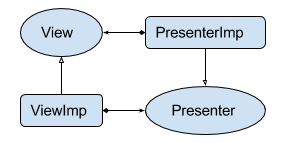
\includegraphics[width=0.5\textwidth, trim={7cm, 7cm, 11cm, 7cm}]{mvp}
	\caption{MVP interface}
	\label{fig:MVP_image}
\end{figure}

The main packages identified a feature of the application and they contain the triad and other utility classes of the feature, for example a DialogFragment.

Aside all pregius of an architecture like MVP we met some difficulties that require the implementations of workaround or a complex solution for a simple task. 

Our need to isolated firebase from other parts of app forced us to use firebase with some limitation. For example Google I/O 2017 available in a open repository in Github [] app use a more complex MVP architecture but the components dependent a lot on firebase API.

Other disadvantages caused by architecture choices are the several callback communication between component, a simple click in a ViewHolder must pass into an Adapter then a Fragment then a Presenter and finally the Controller. By the way we believe that this strong division of relationship between components is a good investments for the future extension of the app.

In the background the app runs four android Service that act like listener to the status of some data into database. 
The UserMonitorService listen when the status of user change, in particular it monitors the relationship status. 
The GeogiftMonitorService manages the life cycle of Geogifts, it downloads them, registers them into LocationService (a Google API Service for monitor location []) and monitors the status of them, if one is destroyed it unregisters it from the LocationServices. When LocationService triggers a Geogift the GeogiftTransitionService acts, it is an IntentService and it create a notification to the user when he discover a Geogift. 
The last Service is the MessagesMonitorService, it monitors the status of all chats and create notifications when new messages are received, it implements a caching system for the notification. The ChatActivity is binded to it in order to reset this notification counter when user enter into a chat.
